%TC第29.1节练习 4、5
%TC第29.2节练习 2、4、6
%TC第29.3节练习 5
%TC第29.4节练习 2
%%%%%%%%%%%%%%%%%%%%%%%%%%%%%%%%%%%%%%%%%%%%%%%%%%%%%%%%%%%%%%%%
% \documentclass[11pt, a4paper, UTF8]{ctexart}
% %%%%%%%%%%%%%%%%%%%%%%%%%%%%%%%%%%%
% File: preamble.tex
%%%%%%%%%%%%%%%%%%%%%%%%%%%%%%%%%%%

\usepackage[top = 1.5cm]{geometry}

% Set fonts commands
\newcommand{\song}{\CJKfamily{song}} 
\newcommand{\hei}{\CJKfamily{hei}} 
\newcommand{\kai}{\CJKfamily{kai}} 
\newcommand{\fs}{\CJKfamily{fs}}

\newcommand{\me}[2]{\author{{\bfseries 姓名:}\underline{#1}\hspace{2em}{\bfseries 学号:}\underline{#2}}}

% Always keep this.
\newcommand{\noplagiarism}{
  \begin{center}
    \fbox{\begin{tabular}{@{}c@{}}
      请独立完成作业,不得抄袭。\\
      若得到他人帮助, 请致谢。\\
      若参考了其它资料,请给出引用。\\
      鼓励讨论,但需独立书写解题过程。
    \end{tabular}}
  \end{center}
}

% Each hw consists of three parts:
% (1) this homework
\newcommand{\beginthishw}{\part{作业}}
% (2) corrections (Optional)
\newcommand{\begincorrection}{\part{订正}}
% (3) any feedback (Optional)
\newcommand{\beginfb}{\part{反馈}}

% For math
\usepackage{amsmath}
\usepackage{amsfonts}
\usepackage{amssymb}

% Define theorem-like environments
\usepackage[amsmath, thmmarks]{ntheorem}

\theoremstyle{break}
\theorembodyfont{\song}
\theoremseparator{}
\newtheorem*{problem}{题目}


\theoremheaderfont{\kai\bfseries}
\theoremseparator{:}
% \newtheorem*{remark}{注}
\theorempostwork{\bigskip\hrule}
\newtheorem*{solution}{解答}
\theorempostwork{\bigskip\hrule}
\newtheorem*{revision}{订正}

\theoremstyle{plain}
\newtheorem*{cause}{错因分析}
\newtheorem*{remark}{注}

\theoremstyle{break}
\theorempostwork{\bigskip\hrule}
\theoremsymbol{\ensuremath{\Box}}
\newtheorem*{proof}{证明}

\renewcommand\figurename{图}
\renewcommand\tablename{表}

% For figures
% for fig with caption: #1: width/size; #2: fig file; #3: fig caption
\newcommand{\fig}[3]{
  \begin{figure}[htp]
    \centering
      \includegraphics[#1]{#2}
      \caption{#3}
  \end{figure}
}

% for fig without caption: #1: width/size; #2: fig file
\newcommand{\fignocaption}[2]{
  \begin{figure}[htp]
    \centering
    \includegraphics[#1]{#2}
  \end{figure}
}
% \usepackage{float}
% \usepackage{amsmath}
% \usepackage{graphicx}
% \usepackage{listings}
% \usepackage{xcolor}
% \usepackage{enumerate}
\documentclass[11pt, a4paper, UTF8]{ctexart}
%%%%%%%%%%%%%%%%%%%%%%%%%%%%%%%%%%%
% File: preamble.tex
%%%%%%%%%%%%%%%%%%%%%%%%%%%%%%%%%%%

\usepackage[top = 1.5cm]{geometry}

% Set fonts commands
\newcommand{\song}{\CJKfamily{song}} 
\newcommand{\hei}{\CJKfamily{hei}} 
\newcommand{\kai}{\CJKfamily{kai}} 
\newcommand{\fs}{\CJKfamily{fs}}

\newcommand{\me}[2]{\author{{\bfseries 姓名:}\underline{#1}\hspace{2em}{\bfseries 学号:}\underline{#2}}}

% Always keep this.
\newcommand{\noplagiarism}{
  \begin{center}
    \fbox{\begin{tabular}{@{}c@{}}
      请独立完成作业,不得抄袭。\\
      若得到他人帮助, 请致谢。\\
      若参考了其它资料,请给出引用。\\
      鼓励讨论,但需独立书写解题过程。
    \end{tabular}}
  \end{center}
}

% Each hw consists of three parts:
% (1) this homework
\newcommand{\beginthishw}{\part{作业}}
% (2) corrections (Optional)
\newcommand{\begincorrection}{\part{订正}}
% (3) any feedback (Optional)
\newcommand{\beginfb}{\part{反馈}}

% For math
\usepackage{amsmath}
\usepackage{amsfonts}
\usepackage{amssymb}

% Define theorem-like environments
\usepackage[amsmath, thmmarks]{ntheorem}

\theoremstyle{break}
\theorembodyfont{\song}
\theoremseparator{}
\newtheorem*{problem}{题目}


\theoremheaderfont{\kai\bfseries}
\theoremseparator{:}
% \newtheorem*{remark}{注}
\theorempostwork{\bigskip\hrule}
\newtheorem*{solution}{解答}
\theorempostwork{\bigskip\hrule}
\newtheorem*{revision}{订正}

\theoremstyle{plain}
\newtheorem*{cause}{错因分析}
\newtheorem*{remark}{注}

\theoremstyle{break}
\theorempostwork{\bigskip\hrule}
\theoremsymbol{\ensuremath{\Box}}
\newtheorem*{proof}{证明}

\renewcommand\figurename{图}
\renewcommand\tablename{表}

% For figures
% for fig with caption: #1: width/size; #2: fig file; #3: fig caption
\newcommand{\fig}[3]{
  \begin{figure}[htp]
    \centering
      \includegraphics[#1]{#2}
      \caption{#3}
  \end{figure}
}

% for fig without caption: #1: width/size; #2: fig file
\newcommand{\fignocaption}[2]{
  \begin{figure}[htp]
    \centering
    \includegraphics[#1]{#2}
  \end{figure}
}
%\usepackage{clrscode3e}
\usepackage{float}
\usepackage{enumerate}
\usepackage{amstext}
\usepackage{amsfonts}
\usepackage{amsmath}
\title{机器学习导论}
\author{殷天润}
\date{\today}
\begin{document}

                                                                                                                

%%%%%%%%%%%%%%%%%%%%%%%%%%%%%%%%%%%%%%%%%%%%%%%%%%%%%%%%%%%%%%%%
%                       Homework START!                        %
%%%%%%%%%%%%%%%%%%%%%%%%%%%%%%%%%%%%%%%%%%%%%%%%%%%%%%%%%%%%%%%%
%%%%%%%%%%%%%%%%%%%%
\section {机器学习导论}

\begin{center} 姓名:殷天润 ~~学号:171240565\end{center}
\begin{problem}[ML problem 1]
	[20pts] Naive Bayes Classifier

		
	We learned about the naive Bayes classifier using the "property conditional independence hypothesis". Now we have a data set as shown in the following table:
	\begin{table}[htp]
		\centering
		\caption{Dataset}\label{tab:aStrangeTable}
	\begin{tabular}{c|ccccc}
		\hline 
		& $x_1$ & $x_2$ & $x_3$ & $x_4$ & $y$ \\ 
		\hline 
	Instance1	& 1 & 1 & 1 & 0 & 1 \\ 
		\hline 
	Instance2	& 1 & 1 & 0 & 0 & 0 \\ 
		\hline 
	Instance3	& 0 & 0 & 1 & 1 & 0 \\ 
		\hline 
	Instance4	& 1 & 0 & 1 & 1 & 1 \\ 
		\hline 
	Instance5	& 0 & 0 & 1 & 1 & 1 \\ 
		\hline 
	\end{tabular}
	\end{table} 
	

		(1) [10pts]  Calculate: $\Pr\{ y=1 | \mathbf{x}=(1,1,0,1) \}$ and $\Pr\{ y=0 | \mathbf{x}=(1,1,0,1) \}$.
		
		(2) [10pts] After using Laplacian Correction, recalculate the value in the previous question.
		
\end{problem}
\begin{solution}
\begin{enumerate}
\item \begin{enumerate}
\item \begin{itemize}
\item P(y=1)=$\frac{3}{5}$=0.6
\item P(y=0)=$\frac{2}{5}$=0.4
\end{itemize}
\item \begin{itemize}
	\item P($x_1=1|y=1$)=$\frac{2}{3}$
	\item P($x_1=1|y=0$)=$\frac{1}{2}$
\end{itemize}
\item \begin{itemize}
	\item P($x_2=1|y=1$)=$\frac{1}{3}$
	\item P($x_2=1|y=0$)=$\frac{1}{2}$
\end{itemize}
\item \begin{itemize}
	\item P($x_3=0|y=1$)=$0$
	\item P($x_3=0|y=0$)=$\frac{1}{2}$
\end{itemize}
\item \begin{itemize}
	\item P($x_4=1|y=1$)=$\frac{2}{3}$
	\item P($x_4=1|y=0$)=$\frac{1}{2}$
\end{itemize}
\end{enumerate}
	所以:
	\begin{itemize}
\item $Pr\{ y=1 | \mathbf{x}=(1,1,0,1) \}=P(y=1)\times P(x_1=1|y=1)\times P(x_2=1|y=1)\times P(x_3=0|y=1) \times P(x_4=1|y=1)=0$
\item $Pr\{ y=0 | \mathbf{x}=(1,1,0,1) \}=P(y=0)\times P(x_1=1|y=0)\times P(x_2=1|y=0)\times P(x_3=0|y=0) \times P(x_4=1|y=0)=0.025$
	\end{itemize}
\item 使用拉普拉斯修正:\begin{enumerate}
	\item \begin{itemize}
	\item P(y=1)=$\frac{3+1}{5+2}$=0.57142
	\item P(y=0)=$\frac{2+1}{5+2}$=0.42857
	\end{itemize}
	\item \begin{itemize}
		\item P($x_1=1|y=1$)=$\frac{2+1}{3+2}$=0.6
		\item P($x_1=1|y=0$)=$\frac{1+1}{2+2}$=0.5
	\end{itemize}
	\item \begin{itemize}
		\item P($x_2=1|y=1$)=$\frac{1+1}{3+2}$=0.4
		\item P($x_2=1|y=0$)=$\frac{1+1}{2+2}$=0.5
	\end{itemize}
	\item \begin{itemize}
		\item P($x_3=0|y=1$)=$\frac{0+1}{3+2}$=0.2
		\item P($x_3=0|y=0$)=$\frac{1+1}{2+2}$=0.5
	\end{itemize}
	\item \begin{itemize}
		\item P($x_4=1|y=1$)=$\frac{2+1}{3+2}$=0.6
		\item P($x_4=1|y=0$)=$\frac{1+1}{2+2}$=0.5
	\end{itemize}
	\end{enumerate}
		所以:
		\begin{itemize}
	\item $Pr\{ y=1 | \mathbf{x}=(1,1,0,1) \}=P(y=1)\times P(x_1=1|y=1)\times P(x_2=1|y=1)\times P(x_3=0|y=1) \times P(x_4=1|y=1)=0.016457$
	\item $Pr\{ y=0 | \mathbf{x}=(1,1,0,1) \}=P(y=0)\times P(x_1=1|y=0)\times P(x_2=1|y=0)\times P(x_3=0|y=0) \times P(x_4=1|y=0)=0.026785$
		\end{itemize}
\end{enumerate}
    
\end{solution}





\begin{problem}[ML problem 2]
	[20pts] Bayes Optimal Classifier

	For a binary classification task, when data in the two classes satisfies Gauss distribution and have the same variance, please prove that LDA can produce the bayes optimal classifier.
\end{problem}
\begin{solution}


\end{solution}
%\newpage
\begin{problem}[ML problem 3]
	[60pts] Ensemble Methods in Practice
	
	Due to their outstanding performance and robustness, ensemble methods are very popular in machine community. In this experiment we will practice ensemble learning methods based on two classic
	ideas: Boosting and Bagging.
	
	In this experiment, we use an UCI dataset Adult. You can refer to the link\footnote{http://archive.ics.uci.edu/ml/datasets/Adult} to see the data description and download the dataset.
	
	Adult is an class imbalanced dataset, so we select AUC as the performance measure. You can adopt sklearn to calculate AUC.
	
(1) [10pts] You need finish the code in Python, and only have two files: AdaBoost.py, RandomForestMain.py. (The training and testing process are implemented in one file for each algorithm.)
	
(2) [40pts] The is experiment requires to finish the following methods:
	
		\begin{itemize}
			\item Implement AdaBoost algorithm according to the Fig(8.3), and adopt decision tree as the base learner (For the base learner, you can import sklearn.)
			\item  Implement Random Forest algorithm. Please give a pseudo-code in the experiment report.
			\item According to the AdaBoost and random forest, analysis the effect of the number of base learners on the performance. Specifically, given the number of base learners, use 5-fold cross validation to obtain the AUC. The range of the number of base learners is decided by yourself.
			\item Select the best number of base classifiers for AdaBoost and random forests, and obtain the AUC in the test set.
		\end{itemize}

(3) [10pts] In the experimental report, you need to present the detail experimental process. The experimental report needs to be hierarchical and organized, so that the reader can understand the purpose, process and result of the experiment.
		
\end{problem}

\begin{solution}
	
\end{solution}




%\begin{problem}[ML problem 5]

	%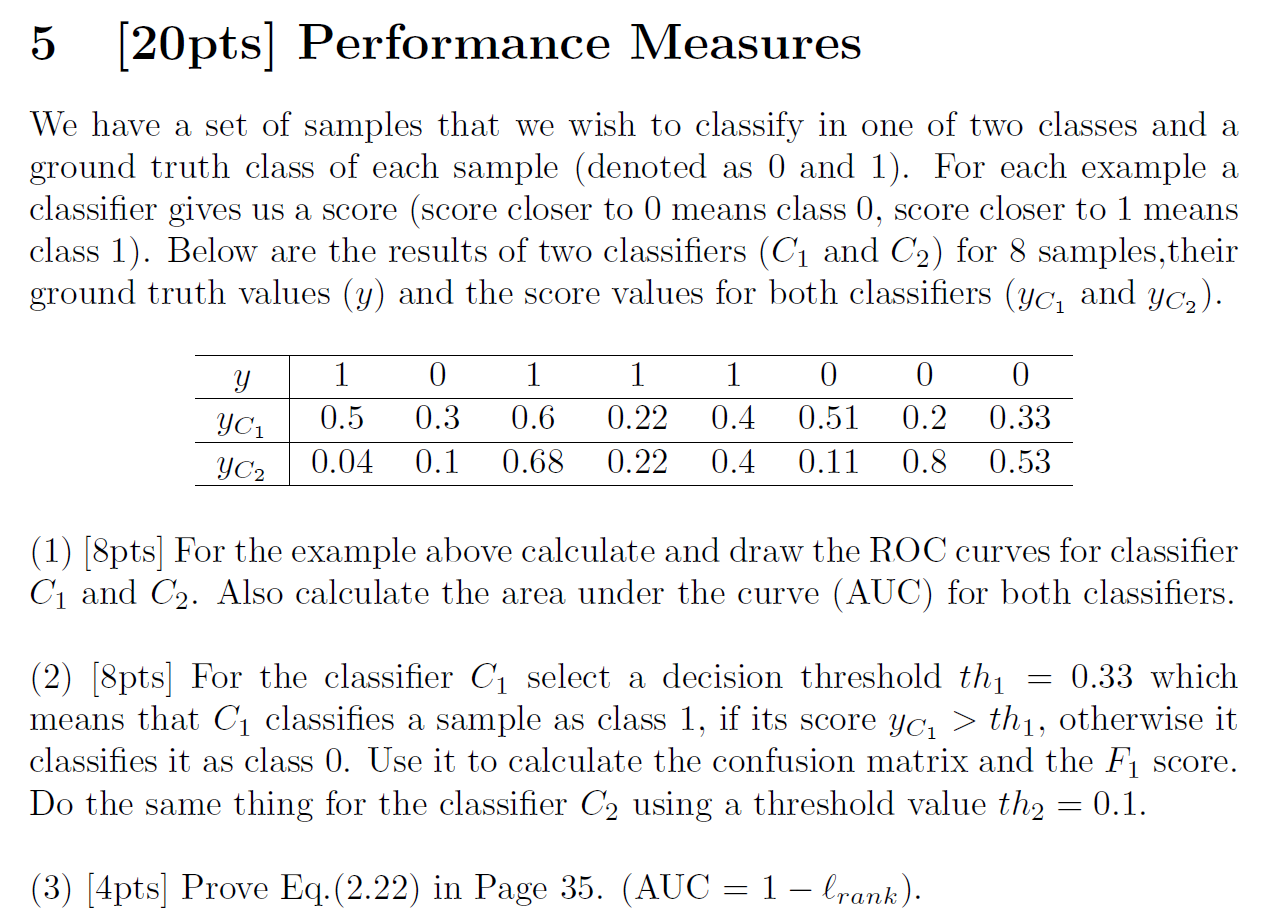
\includegraphics[scale=0.3]{5-p.png}

%\end{problem}
%\newpage
%\begin{solution}
   
%\end{solution}





%\begin{problem}[ML problem 6]
	
%\end{problem}
%\begin{solution}
    
%\end{solution}
%%%%%%%%%%%%%%%%%%%%%%%%%%%%%%%%%%%%%%%%%%%%%%%%%%%%%%%%%%%%%%%%
%                      Correction START!                       %
%%%%%%%%%%%%%%%%%%%%%%%%%%%%%%%%%%%%%%%%%%%%%%%%%%%%%%%%%%%%%%%%
%\begincorrection
%%%%%%%%%%%%%%%%%%%%
%\begin{problem}[]

%\end{problem}

%\begin{cause}
%
%\end{cause}

%\begin{revision}

%\end{revision}
%%%%%%%%%%%%%%%%%%%%
%\newpage
%%%%%%%%%%%%%%%%%%%%





%%%%%%%%%%%%%%%%%%%%%%%%%%%%%%%%%%%%%%%%%%%%%%%%%%%%%%%%%%%%%%%%
%                       Feedback START!                        %
%%%%%%%%%%%%%%%%%%%%%%%%%%%%%%%%%%%%%%%%%%%%%%%%%%%%%%%%%%%%%%%%
%\beginfb
%\begin{itemize}
%
%\end{itemize}





%%%%%%%%%%%%%%%%%%%%%%%%%%%%%%%%%%%%%%%%%%%%%%%%%%%%%%%%%%%%%%%%
%                        Homework END!                         %
%%%%%%%%%%%%%%%%%%%%%%%%%%%%%%%%%%%%%%%%%%%%%%%%%%%%%%%%%%%%%%%%
\end{document}
